\section{Experimental Setup}
\label{sec:setup}

Athough the detection techniques described in \ref{sec:detection} are in principle adaptable to similar data, the image data used in this thesis is captured using a specific setup. 

The setup uses the \emph{Fastcam Mini UX} in combination with a \emph{Olympus LMPlan IR 50X / 0.55} microscope objective lens as well as a seperate focussing lens to capture images of the droplets.
Together with a parallel light source, this setup forms a microscope with a large magnification factor, which is necessary to capture the droplets in sufficient detail considering their expected size of \SIrange{1}{30}{\micro\meter} \cite{kapplAkustischInduzierteVernebelung2022}.

The SAW device together with a liquid reservoir is placed next to the light source and the camera so that the droplet droplet stream is illuminated from the side. An image of the setup is shown in Figure~\ref{fig:setup}.

Images are taken at a resolution of \qtyproduct{1280 x 1024}{\pixel} and a frame rate of \SI{50}{\hertz}. The framerate is kept low to enable capturing data over a longer period of time without saturating the memory of the camera, since the droplets are not constantly in the field of view of the microscope. 

\begin{figure}[htbp]
    \centering
    \makebox[\textwidth][c]{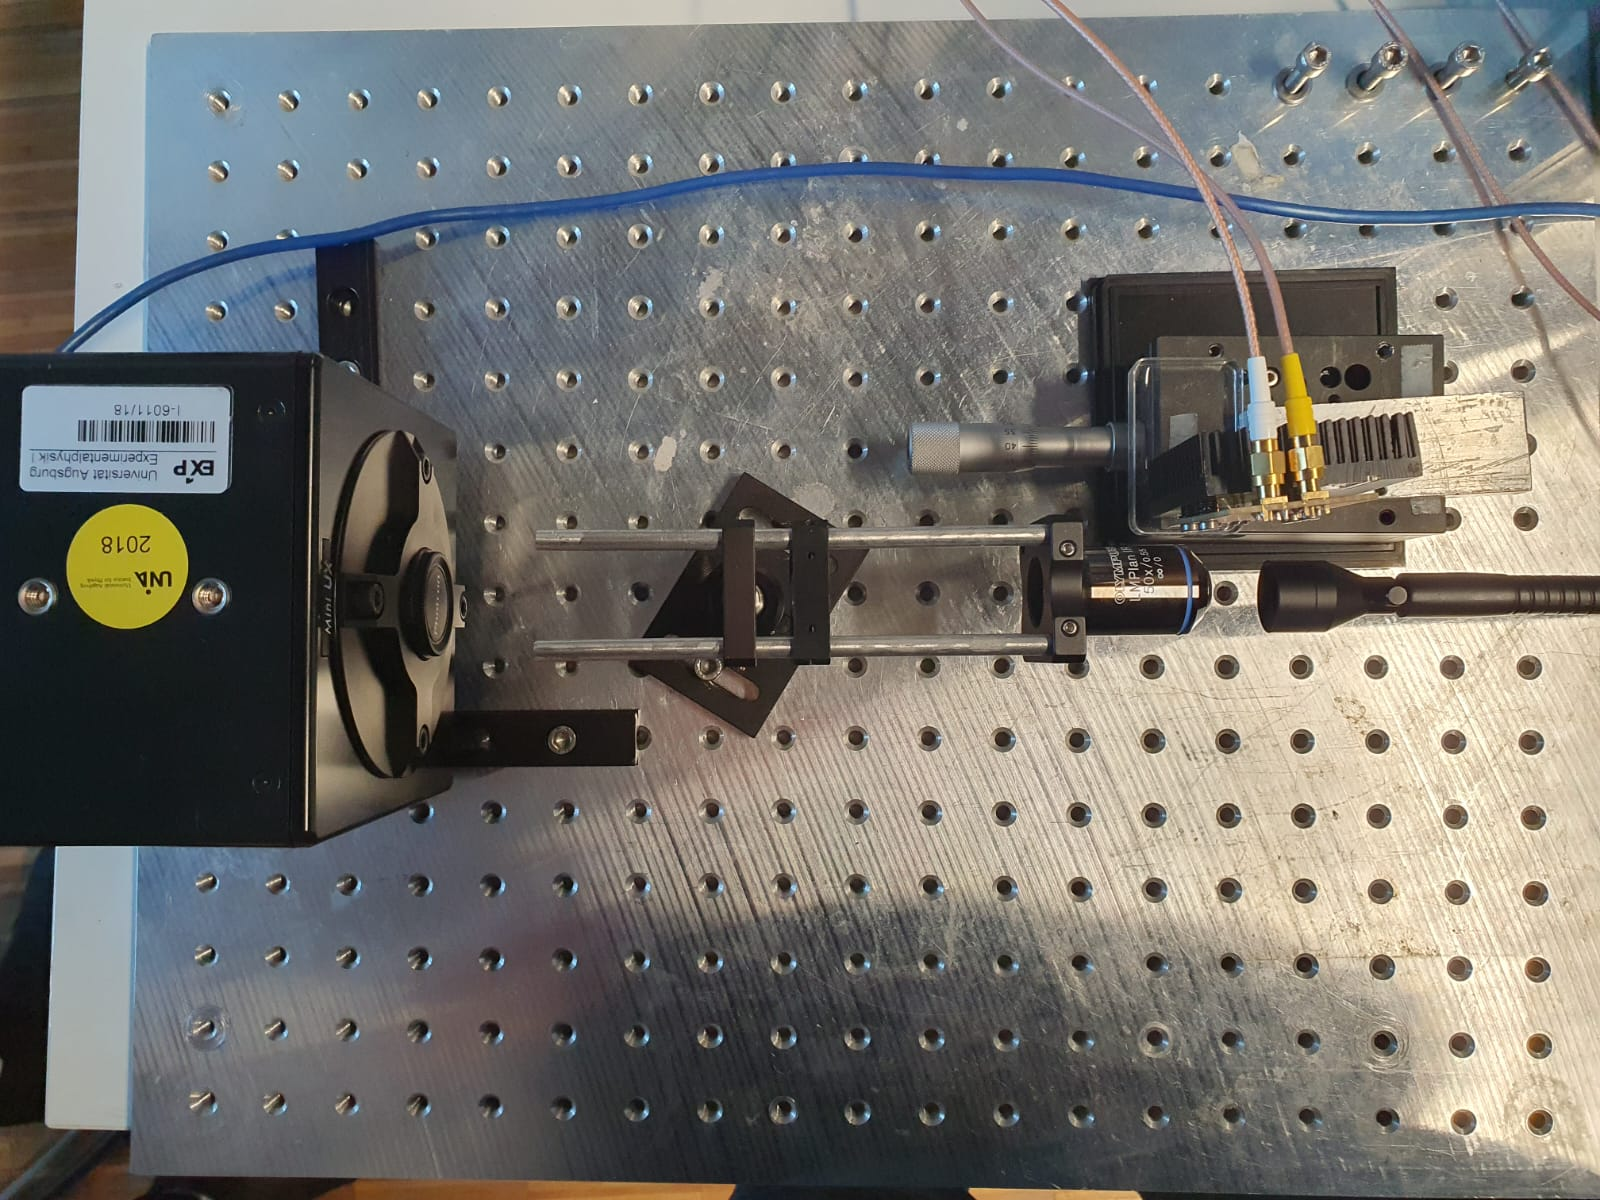
\includegraphics[width=0.9\textwidth]{images/0c35c5ed-b77b-4d8d-b30f-b23403bd04d0.JPG}}
    \vspace{0.2cm}
    \caption{Image of the measurement setup. From left to right the high speed camera, the focusing lens and objective lens, the SAW device and the liquid reservoir as well as the light source are visible.}
    \label{fig:setup}
\end{figure}